\documentclass[a4paper, 16pt]{article}
\usepackage[UTF8]{ctex}
\usepackage{geometry}
\usepackage{graphicx}
\usepackage{setspace}
\usepackage{float}
\usepackage{listings}
\usepackage{xcolor}
\lstset{
    numbers=left, 
    numberstyle= \tiny, 
    keywordstyle= \color{ blue!70},
    commentstyle= \color{red!50!green!50!blue!50}, 
    frame=shadowbox, % 阴影效果
    rulesepcolor= \color{ red!20!green!20!blue!20} ,
    escapeinside=``, % 英文分号中可写入中文
    xleftmargin=5em,xrightmargin=5em, aboveskip=2em,
    framexleftmargin=2em
} 
\geometry{left = 1.0 cm, right = 1.0cm, top = 2.0cm, bottom = 2.0cm	}
\title{编译原理第六章(二)}
\author{李鹏辉}

\begin{document}
\maketitle
1.(6.3.1)确定下列声明序列中各个标志符的类型和相对地址
\lstset{language=C}
\begin{lstlisting}
float x;
record {float x; float y} p;
record {int tag; float x; float y} q;
\end{lstlisting}

\begin{table}[H]
\centering
\begin{tabular}{c|c|c|c}
\hline
\hline
  &$id$& $type$ & $offset$ \\
\hline
(0) & x & float & 0  \\
\hline
(1) & x & float & 0  \\
    & y & float & 8 \\
    & p & record & 8 \\
\hline 
 (3)& tag& float & 0 \\
    & x & float & 4 \\
    & y & float &12 \\
    & q & record& 20 \\
\hline
\end{tabular}
\end{table}



2.(6.4.3)使用图6-22的翻译方案翻译下列赋值语句

1) $x = a[i] + b[j]$
假设a,b为int类型
\begin{figure}[H]
\centering
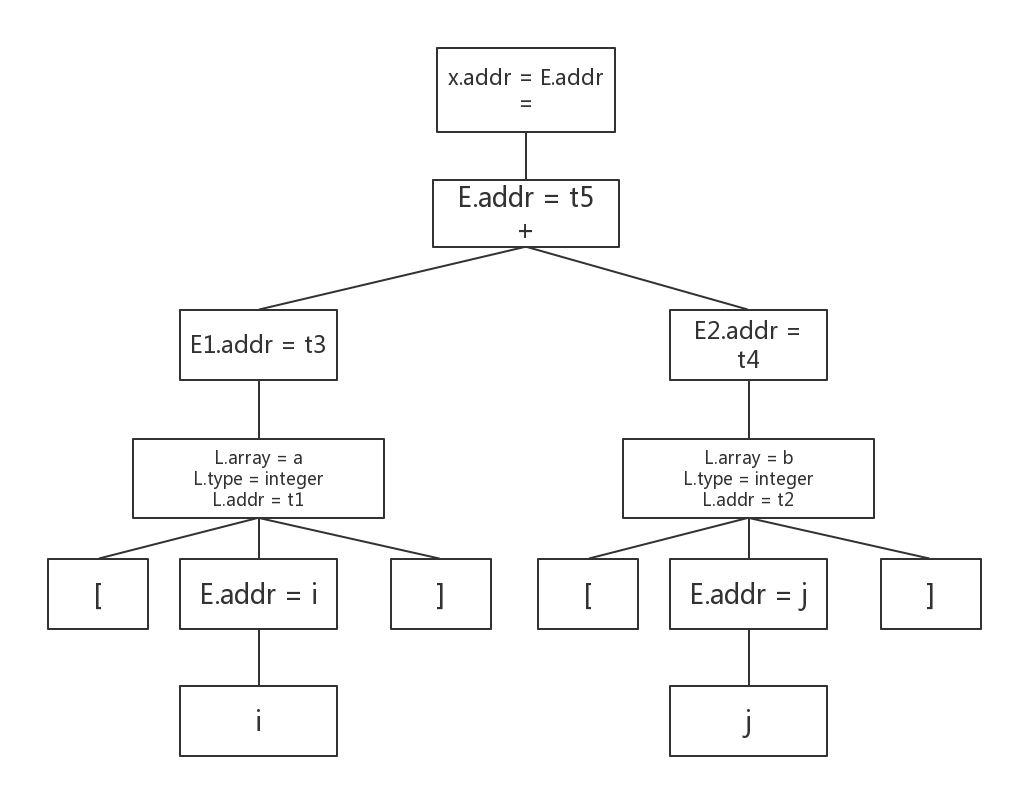
\includegraphics[scale=0.3]{chapter6_hw2_1}
\caption{翻译 $x = a[i] + b[j]$}
\end{figure}
三地址代码如下:

$t_1 = 4* i$

$t_2 = 4*j$

$t_3 = a[t_1]$

$t_4 = b[ t_2]$

$t_5 = t_3 + t_4$

$x = t_5$\\


2) $x = a[i][j] + b[i][j]$
假设a,b为int类型
\begin{figure}[H]
\centering
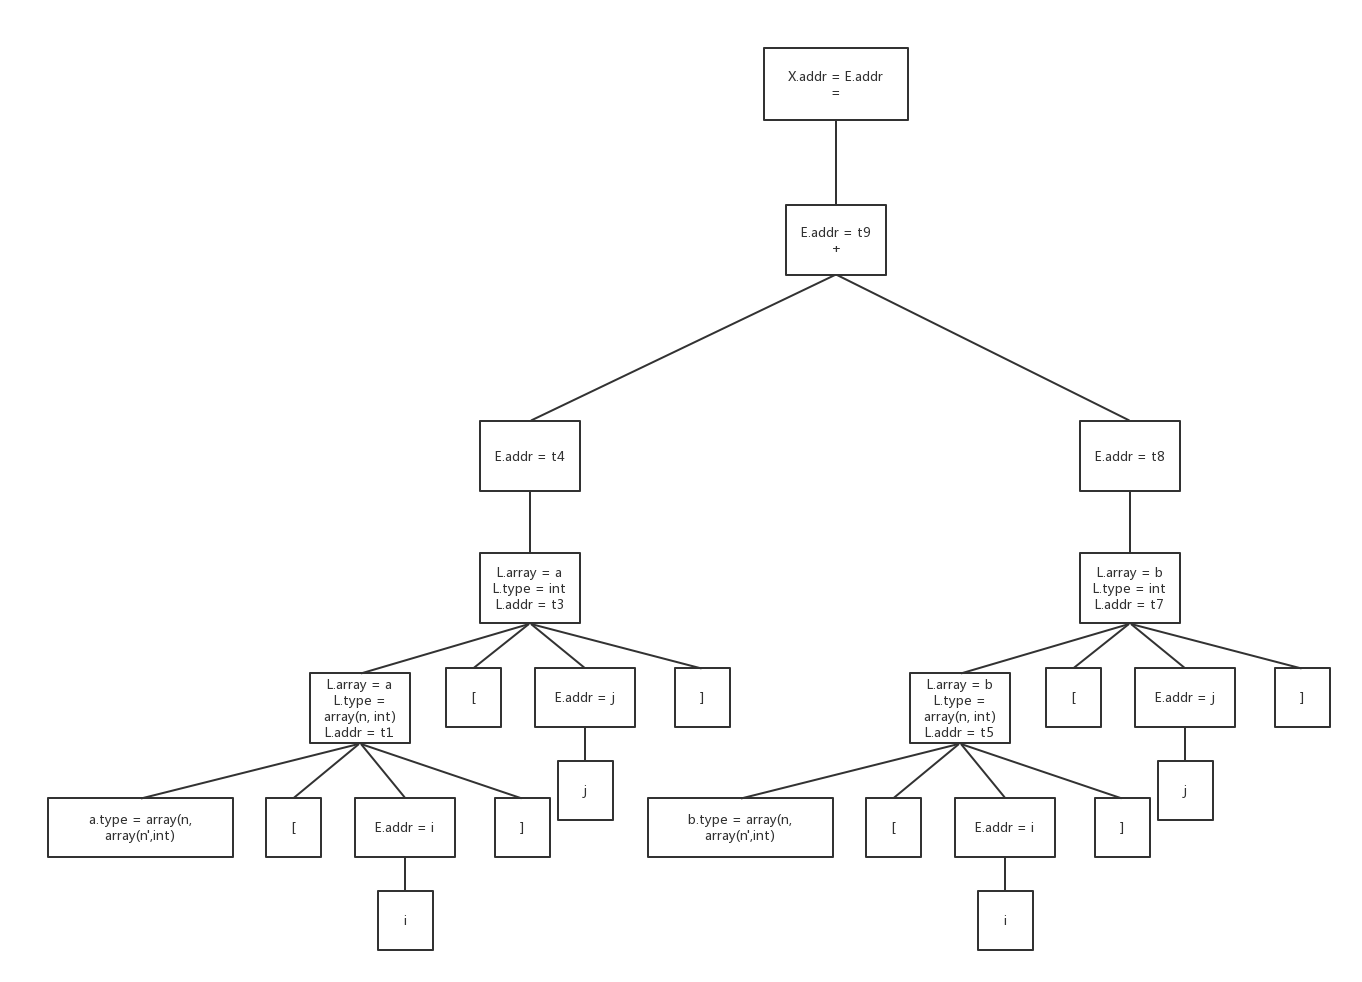
\includegraphics[scale=0.3]{chapter6_hw2_2}
\caption{翻译 $x = a[i][j] + b[i][j]$}
\end{figure}

三地址代码如下:

$t_1 = 4*n'* i$

$t_2 = 4*j$

$t_3 = t_1 + t_2$

$t_4 = a[t_3]$

$t_5 = 4*n''* i$

$t_6 = 4*j$

$t_7 = t_5 + t_6$

$t_8 = a[t_7]$

$t_9 = t_8 + t_4$

$x = t_9$\\

3.(6.5.1)假定图6-26中函数widen可以处理图6-25a的层次结构中的所有类型,翻译下列表达式。假定c和d是字符型,s和t是短整型,i和j是整型,x是浮点型.

$char \;\; c,\; d; short\;\; s,\;t; int \; \; i,\;j; float \; \;x;$

1) $x = s + c$

$tmp_1 = s + (short)c$

$x = (flost) tmp_1$\\

2) $i = s + c$

$tmp_1 = s + (short)c$

$i = (int) tmp_1$\\

3) $x = (s+c) * (t+d)$

$tmp_1 = s + (short)c$

$tmp_2 = t + (short)d$

$x = (float) tmp_1 * tmp_2$
\end{document}